% !Mode:: "TeX:UTF-8" (encoding info for WinEdt)
\section{Connexion à une base de données externe}
 Lors du premier démarrage Elexis crée d'emblée une base de donnée HSQL locale. Il est par contre tout à fait possible de se connecter à une autre base de données qui se trouve sur n'importe quel autre ordinateur dans le réseau ou même en se branchant à travers Internet ( pour des raisons de sécurité ceci est seulement conseillé si certaines conditions de protection sont remplis). Créez d'abord une base de données vide sur l'ordinateur qui devait servir comme serveur. Supposons par ex ce serveur ait l'adresse IP 192.168.0.2. Pour l'installation de mysql l'installation se fait comme suit, pour d'autres types de base de données l'installation se fait en analogie.

\subsection{création d'une base de données}
Veuillez vous connecter à votre serveur et introduisez ce qui suit :
\begin{itemize}
 \item mysql -u root
\end{itemize}

ceci ouvre la console de mysql (si vous l'avez correctement installé).
Veuillez introduire en suite : 
\begin{itemize}
 \item create database elexistest;
\item grant all on elexis.* to testuser\@'\%' identified by 'testelexis';
\end{itemize}




(Il  n'est naturellement pas interdit de choisir un autre nom de la base de donnée et un autre nom d'utilisateur ou un autre mot de passe.)

Démarrez ensuite Elexis et choisissez dans le menu fichier  \textit{Connexion}.

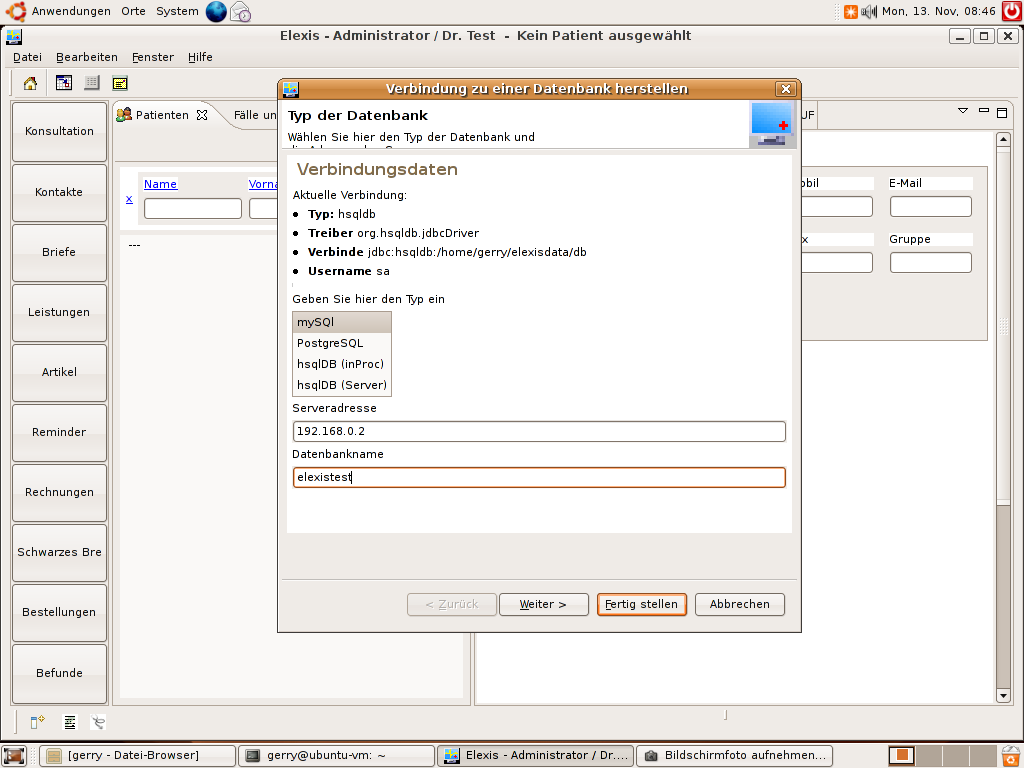
\includegraphics[width=4in]{images/verbindung1.png}
% verbindung1.png: 1024x768 pixel, 72dpi, 36.12x27.09 cm, bb=0 0 1024 768

Entrez le type de base de données (ici mysql), l'adresse u serveur (ici 192.168.0.2) ou son adresse internet (par ex testserveur.elexis.ch) de même que le nom de la base de données (ici elexistest) et cliquez sur \textit{suivre}.

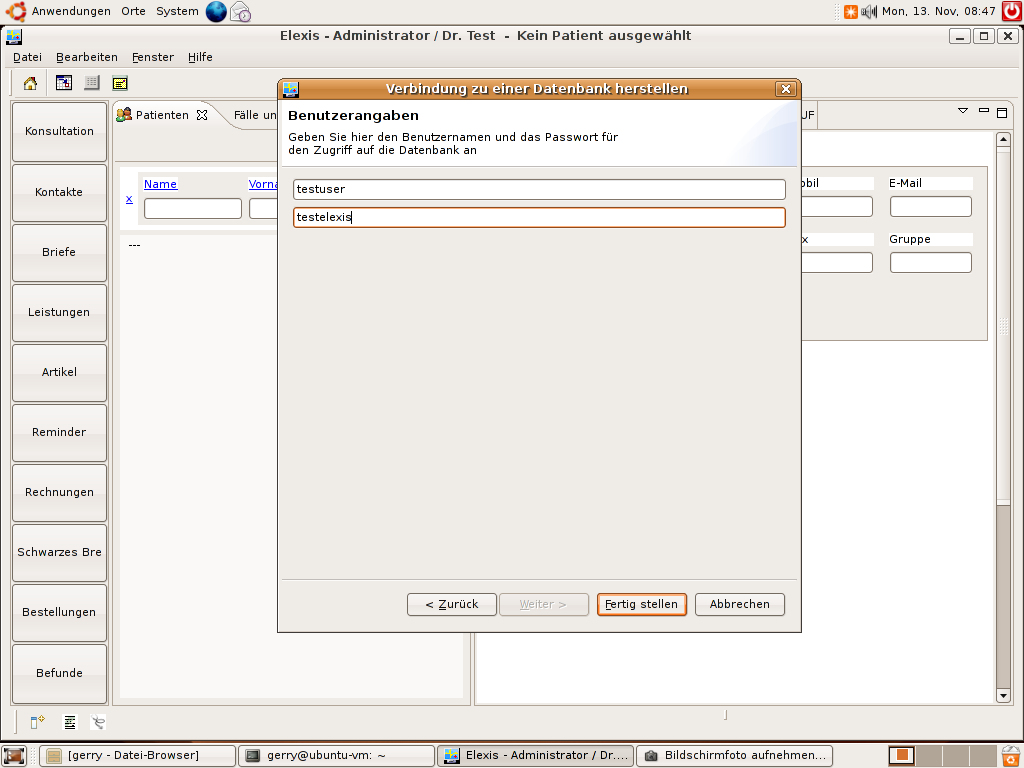
\includegraphics[width=4in]{images/verbindung2.png}
% verbindung2.png: 1024x768 pixel, 72dpi, 36.12x27.09 cm, bb=0 0 1024 768

Veuillez introduire dans la ligne supérieure le nom de l'utilisateur de la base de données (ici testuser) et dans la ligne inférieure le mot de passe (ici testelexis) et cliquez ensuite sur \textit{terminer}.

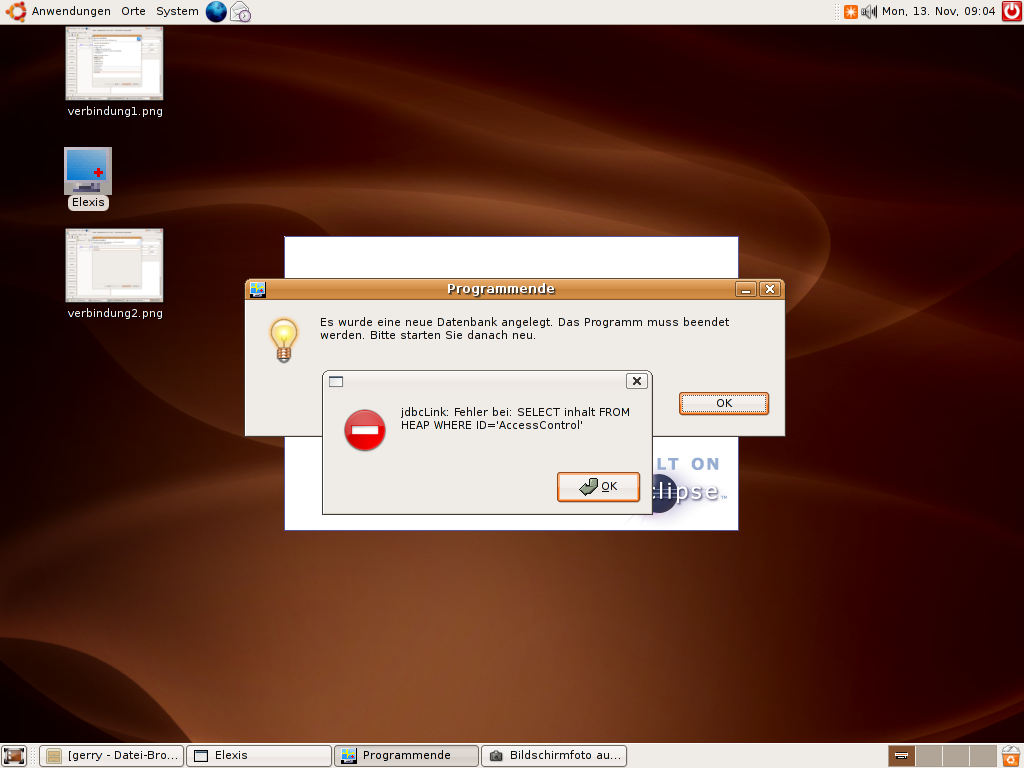
\includegraphics[width=4in]{images/verbindung3.png}
% verbindung3.png: 1024x768 pixel, 72dpi, 36.12x27.09 cm, bb=0 0 1024 768

Souvent quelques messages d'erreur apparaissent que vous pouvez ignorer. Finalement il faudra restarter encore une fois le  program.

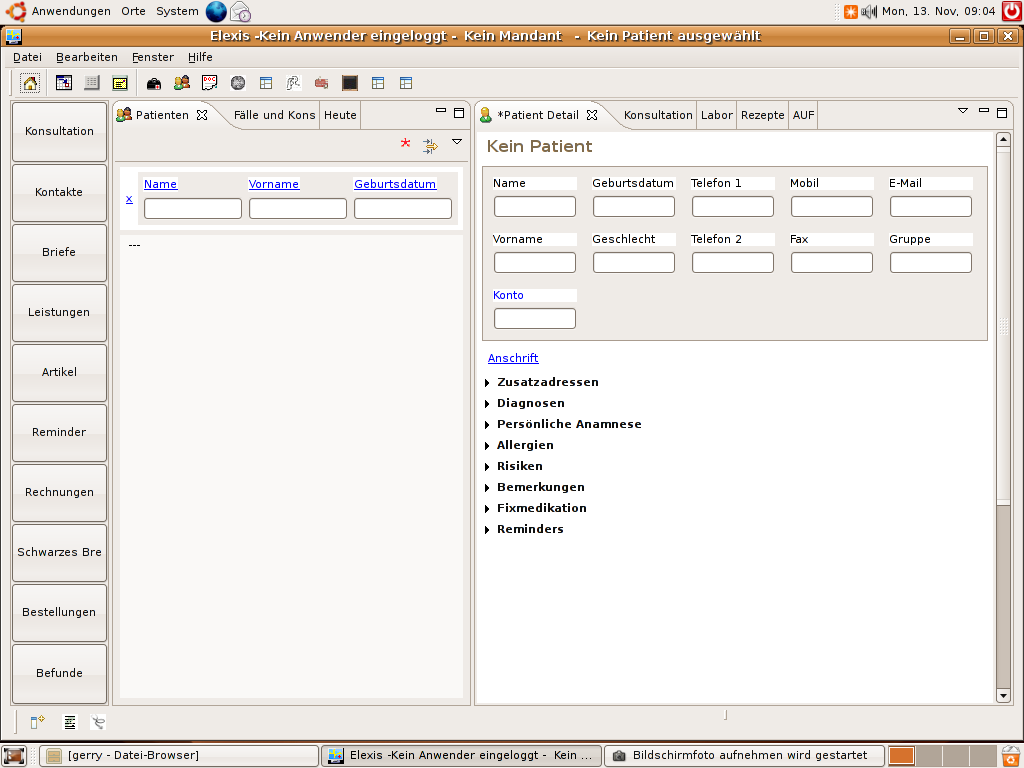
\includegraphics[width=4in]{images/verbindung4.png}
% verbindung4.png: 1024x768 pixel, 72dpi, 36.12x27.09 cm, bb=0 0 1024 768


 Maintenant vous pouvez vous brancher avec le nom d'utilisateur \textit{Administrator} et avec le mot de passe \textit{admin} dans le système de Elexis que vous venez de créer. 